\newpage
\section{Consuntivo di periodo} \label{ConsuntivoPeriodo}

In questa sezione viene effettuato un confronto fra le ore ed il costo preventivati con quelli riscontrati effettivamente durante i periodi del ciclo di sviluppo, oltre ad eventuali scostamenti sulla pianificazione. Viene poi riportato, nella sezione seguente, il preventivo a finire.
Viene inoltre analizzato e riportato il bilancio che potrà essere:
\begin{itemize}
	\item \textbf{positivo}: se il consuntivo risulta inferiore o equivalente al preventivo;
	\item \textbf{negativo}: se il consuntivo risulta superiore al preventivo.
\end{itemize}

\subsection{Analisi dei requisiti}
\subsubsection{Consuntivo}
Di seguito è riportata la tabella riassuntiva per il consuntivo del primo periodo.
\begin{table}[h!]
	\centerline{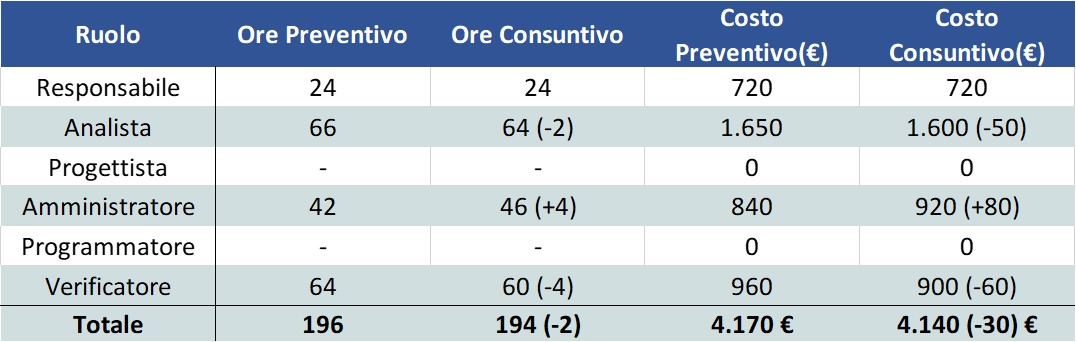
\includegraphics[scale=0.55]{img/Preventivo/Consuntivo/AnalisiRequisitiConsuntivo.jpg}}
	\caption{Consuntivo: Analisi dei requisiti}
\end{table}

\subsubsection{Conclusioni}
Durante questo primo periodo non ci sono state grandi discordanze rispetto a quanto pianificato. Sono state necessarie alcune ore aggiuntive agli \adms{} in contrapposizione agli \anas{} e si è inoltre rivelato necessario un impegno minore da parte dei \vers{} rispetto a quanto preventivato.\\
Questi fattori hanno favorito un risparmio rispetto al costo inizialmente preventivato pari a \EUR{30} e quindi il bilancio di questo primo periodo risulta positivo.

\subsection{Analisi dei requisiti in Dettaglio}
\subsubsection{Conclusioni}
Durante questo periodo non sono state necessarie correzioni al preventivo iniziale, perciò non verrà riportata alcuna tabella di consuntivo. Si può quindi far riferimento al \hyperref[PreventivoAnalisiRequisitiDettaglio]{preventivo} relativo a questo periodo per completezza. \\
È stato necessario, tuttavia, far avanzare la data di milestone interna, che definisce la fine di questo periodo, dal giorno 26 al giorno 29 Aprile. Si rimanda all'\hyperref[RiscontroAnalisiDettaglio]{attualizzazione dei rischi} di questo periodo per completezza.

\newpage
\subsection{Prototipazione}
\subsubsection{Consuntivo}
Di seguito è riportata la tabella riassuntiva per il consuntivo di questo periodo.
\begin{table}[h!]
	\centerline{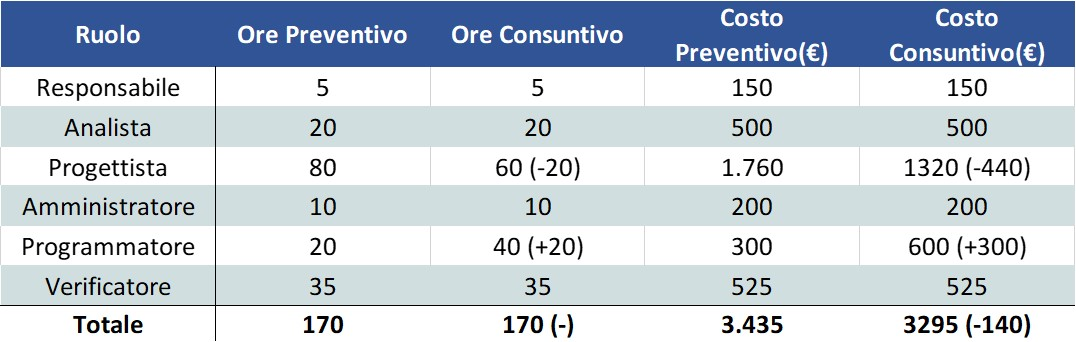
\includegraphics[scale=0.55]{img/Preventivo/Consuntivo/PrototipazioneConsuntivo.jpg}}
	\caption{Consuntivo: Prototipazione}
\end{table}

\subsubsection{Conclusioni}
Durante questa fase si sono rese necessarie ore aggiuntive ai \progrs{}: oltre ad essere frutto di una previsione errata in fase di preventivo, questo scostamento è molto probabilmente dovuto all'inesperienza con alcune delle tecnologie adottate e quindi si prevede che in futuro sarà meno accentuato rispetto a quanto preventivato. Le ore destinate ai \progrs{} sono state invece compensate da un minor impegno da parte dei \progs{}. Nel complesso, i fattori appena analizzati, hanno portato ad un risparmio pari a \EUR{140} rispetto al preventivo di periodo; il bilancio di questo periodo risulta quindi positivo. \\ 
Nel \hyperref[PreventivoFinire]{preventivo a finire} è possibile notare come il consuntivo di questo periodo abbia causato una modifica al preventivo iniziale totale.